% Limpa cabeçalhos.
% (solução para lidar com a númeração das páginas pré-textuais).
\pagestyle{empty}


% ----------------------------------------------------------
% ELEMENTOS PRÉ-TEXTUAIS
% ----------------------------------------------------------
\renewcommand{\today}{\ifcase \month \or Janeiro\or Fevereiro\or Março\or Abril\or Maio\or Junho\or Julho\or Agosto\or Setembro\or Outubro\or Novembro\or Dezembro\fi/\number \year}
%============================ Início da capa ============================================
\begin{center}
%--------------------------------------------
\begin{figure}[h!]
\parbox{2.5cm}{
\includegraphics[scale=0.15]{ufpi.jpg}}%
\quad
\begin{minipage}{12cm}%
\vspace{1cm}
\textsc{\large UNIVERSIDADE FEDERAL DO PIAUÍ}\\
\textsc{\large CENTRO DE TECNOLOGIA}\\
\textsc{\large BACHARELADO EM ENGENHARIA ELÉTRICA}\\
\end{minipage} %
\end{figure}
\vspace{4cm}
%nome do aluno
\textbf{\large FRANCISCO MARCOLINO RODRIGUES FILHO}\\
\vspace{4cm}
%título tcc
\textbf{\large ESTUDO E IMPLEMENTAÇÃO DE ALGORITMO INTELIGENTE PARA RESOLUÇÃO DE LABIRINTO COM ROBÔ AUTÔNOMO DIFERENCIAL MICROMOUSE}\\
\vfill
\textsc{\large teresina - piauí, \today}\\
\end{center}
\clearpage
%=========================== Fim da capa ===================================================


%============================ Início da página de rosto ============================================
\begin{center}
%----------------------------------------------------
\textbf{\Large FRANCISCO MARCOLINO RODRIGUES FILHO}
\par
\vspace{4cm}
\textbf{\Large ESTUDO E IMPLEMENTAÇÃO DE ALGORITMO INTELIGENTE PARA RESOLUÇÃO DE LABIRINTO COM ROBÔ AUTÔNOMO DIFERENCIAL MICROMOUSE}
\end{center}
\par
\vspace{4cm}
\hspace*{160pt}\parbox{9cm}{{Trabalho de conclusão de curso apresentado como requisito parcial para a obtenção do título de Bacharel em Engenharia Elétrica, pelo curso de Engenharia Elétrica da Universidade Federal do Piauí - UFPI.}}
\vspace{2cm}
\par\hspace*{160pt}\parbox{10cm}{Orientador: Prof. Dr. Otacílio da Mota Almeida}
%\vspace{-0.3cm}
%\par\hspace*{160pt}\parbox{10cm}{Co-orientador: Nome do Co-orientador}
\vfill
\begin{center}
\textsc{\large teresina - piauí, \today}\\
\end{center}
\newpage
%============================ Fim da página de rosto ============================================

%============================ Início da Ficha Catalográfica ==========================================
% Dados
% \codigo{M217p}
\begin{fichacatalografica}
	\sffamily
	\vspace*{\fill}					% Posição vertical
	\begin{center}					% Minipage Centralizado
		\fbox{\begin{minipage}[t]{10.5cm}		% Largura
				R696e
				\hspace*{0.2cm}
				\parbox[t]{8.3cm}{
					Rodrigues Filho, Francisco Marcolino.
				
					\hspace{0.5cm} \imprimirtitulo~/~\imprimirautor.~--~\imprimirdata.
				
					\hspace{0.5cm} \sumoffset{LastPage}{LastPreContentPage} f.\\
				
					\parbox[t]{9cm}{\hspace{0.5cm}Monografia (Graduação) -- Bacharelado em
					Engenharia Elétrica, Universidade Federal do Piauí, \imprimirdata.}
				
					\hspace{0.5cm} "\imprimirorientadorRotulo~\imprimirorientador"\\
				
					\hspace{0.5cm}
					1. Micromouse (Robótica).
					2. Algoritmo Inteligente.
					3. Labirinto. Flood Fill.
					4. Robótica didática.
					I. Título.
				}
			
				\hspace*{\fill} CDD 629.892
		\end{minipage}}
	\end{center}
\end{fichacatalografica}

\newpage
%============================ Fim da Ficha Catalográfica ==============================================


%============================ Início da folha de aprovação ============================================
\begin{center}
%----------------------------------------------------
\textbf{\Large FRANCISCO MARCOLINO RODRIGUES FILHO}
\par
\vspace{2cm}
\textbf{\Large ESTUDO E IMPLEMENTAÇÃO DE ALGORITMO INTELIGENTE PARA RESOLUÇÃO DE LABIRINTO COM ROBÔ AUTÔNOMO DIFERENCIAL MICROMOUSE}
\end{center}
\par
\vspace{1cm}
\hspace*{160pt}\parbox{9cm}{{Trabalho de conclusão de curso apresentado como requisito parcial para a obtenção do título de Bacharel em Engenharia Elétrica, pelo curso de Engenharia Elétrica da Universidade Federal do Piauí - UFPI.}}
\vspace{1.75cm}
\par\hspace*{160pt}\parbox{10cm}{Orientador: Prof. Dr. Otacílio da Mota Almeida}
%\vspace{-0.3cm}
%\par\hspace*{160pt}\parbox{10cm}{Co-orientador: Nome do Co-orientador}
\vspace{1cm}
\begin{center}
Aprovado em 7 de julho de 2017.
\vspace{1.5cm}

BANCA EXAMINADORA
\vspace{0.01cm}

\begin{figure*}[!htb]
	\begin{center}
		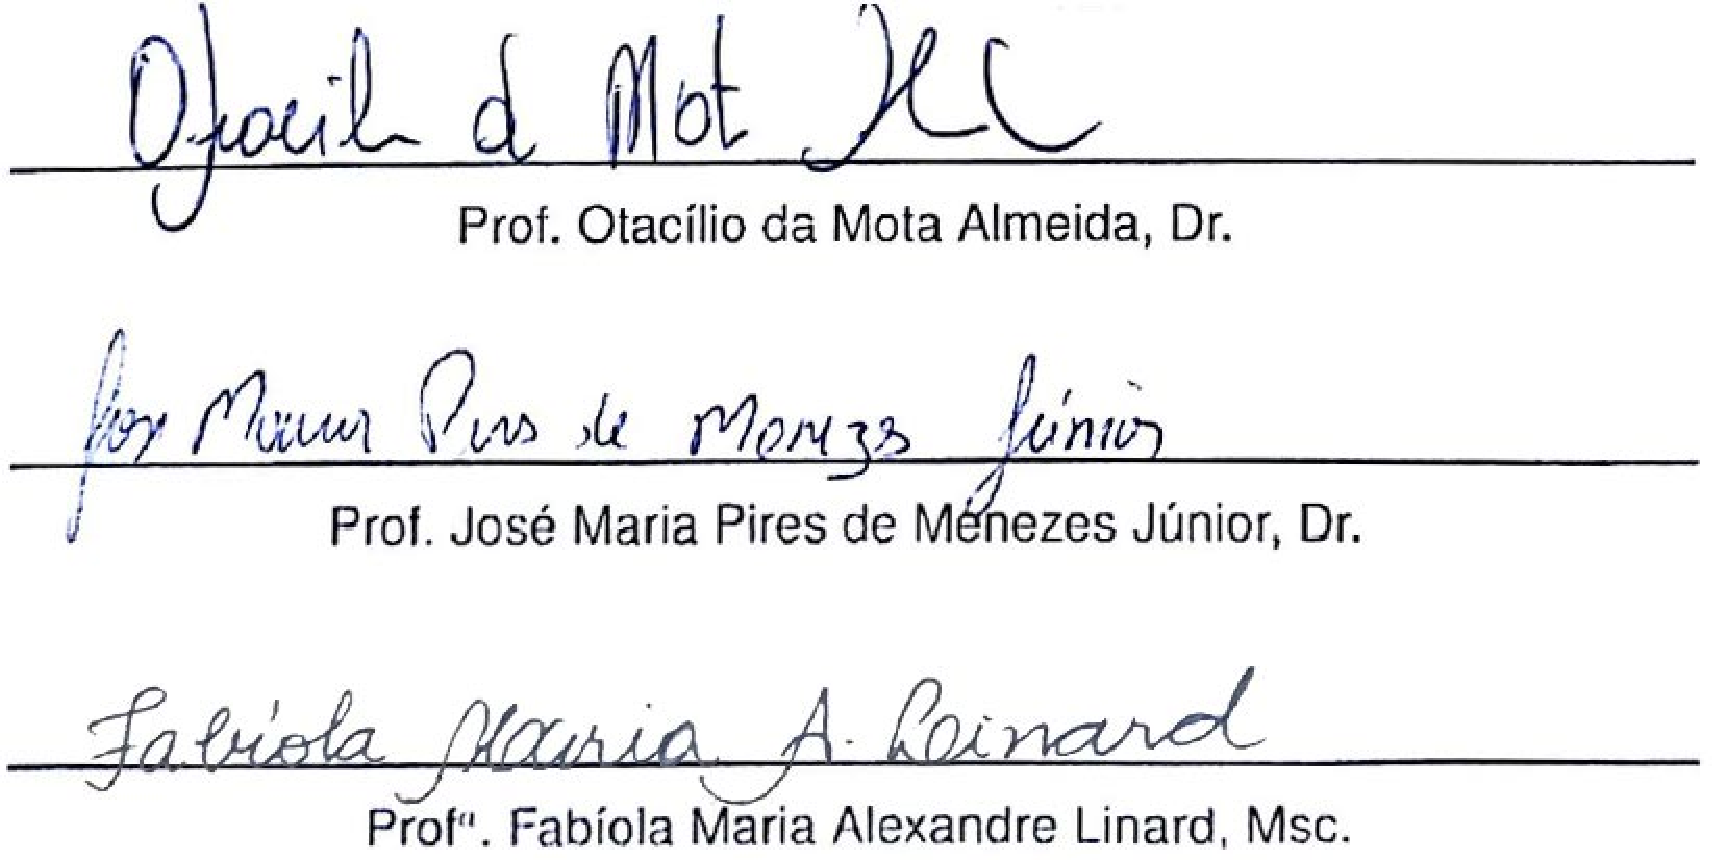
\includegraphics[width=.9\linewidth]{assinaturas.pdf}
	\end{center}
\end{figure*}
%
%\rule{14cm}{1pt}\\
%Prof. Otacílio da Mota Almeida, Dr.
%\vspace{1cm}
%
%\rule{14cm}{1pt}\\
%Prof. José Maria Pires de Menezes Júnior, Dr.
%\vspace{1cm}
%
%\rule{14cm}{1pt}\\
%Prof$^a$. Fabíola Maria Alexandre Linard, Msc.

\end{center}
\clearpage
%============================ Fim da folha de aprovação ============================================

%-------------- AGRADECIMENTO + RESUMO + ABSTRACT ----------------------------------

\noindent{\LARGE\textbf{Agradecimentos}}

A Deus pelos caminhos que até aqui me trouxeram.

À minha família pelo apoio incondicional, pelo suporte sempre prestado e pelo amor a mim dedicado. Meus pais, mesmo à distância, não mediram esforços para me apoiar. Agradeço a eles pela confiança prestada.

%À Zafira automática, que já serviu de casa por quatro dias no início do curso.

Aos professores do curso que me ajudaram e guiaram nos momentos de incerteza.

Agradeço em especial ao professor orientador Otacílio da Mota Almeida pela ajuda nesta caminhada, que desde o início do curso me apoiou fortemente. Agradeço a ele, como Tutor, por ter me aceitado como membro do PET - Programa de Educação Tutorial, do curso de Engenharia Elétrica da UFPI, e por ter financiado o Micromouse por conta própria, que possibilitou este trabalho. Afirmo que minha graduação não seria a mesma sem ele.

Aos amigos do PET, à sala do PET, aos trabalhos do PET.

Aos colegas e amigos Fabilo de Arruda Leda e José Genilson Sousa Carvalho, irmãos que ganhei durante a graduação. Sem vocês esta página estaria em branco. Agradeço aos colegas do curso pela amizade criada, e às mães dos meus colegas, que me adotaram nesta caminhada.




\newpage

\vspace*{10pt}
% Resumo
\begin{center}
  \emph{\begin{large}Resumo\end{large}}\label{resumo}
\vspace{2pt}
\end{center}
% Pode parecer estranho, mas colocar uma frase por linha ajuda a organizar e reescrever o texto quando necessário.
% Além disso, ajuda se você estiver comparando versões diferentes do mesmo texto.
% Para separar parágrafos utilize uma linha em branco.
\noindent
  Micromouse é uma competição robótica que teve início nos anos 70 e vem ganhando espaço à medida que as tecnologias de integração em alta densidade, sensores e teoria de controle inteligente avançam. O desafio consiste na resolução de labirinto partindo de um dos cantos até o seu centro, com a utilização de mini robô móvel (Micromouse), no menor tempo possível. O micromouse é um robô com sensores de distância e \emph{encoders} conectados a um microcontrolador, permitindo que o robô se locomova numa direção predefinida por um algoritmo. Dentro do microcontrolador, o controle de trajetória, memória das paredes do labirinto e se situar no mesmo para saber se já chegou ao alvo são executados logicamente. Existem diversos algoritmos de resolução de labirinto com robôs móveis, porém, o mais utilizado é o \textit{Flood Fill}. Com base neste algoritmo, este trabalho propõe uma nova estratégia para implementação de algoritmo inteligente de resolução de labirinto. A ideia é utilizar uma estrutura de dados para armazenar tanto o caminho de ida do robô como o caminho de volta. Para avaliar o desempenho do algoritmo várias simulações foram realizadas e comparadas com o \emph{Flood Fill clássico} resultando em substancial economia de \emph{RAM} que favorece a implementação em tempo real do sistema embarcado no micromouse. A implementação do algoritmo ocorreu da forma esperada, sendo que o percurso do robô num labirinto-teste é o mesmo do simulador. Portanto, este trabalho tem como objetivo a implementação do algoritmo inteligente de resolução de labirinto e do algoritmo de controle de trajetórias em robô micromouse, com características e requisitos necessários para participação em competições de desafios Micromouse.
\par
\vspace{1em}
\noindent\textbf{Palavras-chave:} Micromouse. Algoritmo inteligente. Labirinto. Flood Fill. Robótica didática.
\newpage

% Criei a página do abstract na mão, por isso tem bem mais comandos do que o resumo acima, apesar de serem idênticas.
\vspace*{10pt}
% Abstract
\begin{center}
  \emph{\begin{large}Abstract\end{large}}\label{abstract}
\vspace{2pt}
\end{center}

% Selecionar a linguagem acerta os padrões de hifenação diferentes entre inglês e português.
\selectlanguage{english}
\noindent
Micromouse is a robotic competition that began in the 1970s and is gaining momentum as high density integration technologies, sensors and intelligent control theory advance. The challenge is to solve a labyrinth starting from one of the corners to its center, using a mini mobile robot (Micromouse) in the shortest possible time. The micromouse is a robot with distance sensors and \ emph {encoders} connected to a microcontroller, allowing the robot to move in a predefined direction by an algorithm. Inside the microcontroller, the control of trajectory, memory of the walls of the labyrinth and to be in the same to know if already reached the target are executed logically. There are several labyrinth resolution algorithms with mobile robots, however, the most commonly used is \ textit {Flood Fill}. Based on this algorithm, this work proposes a new strategy for implementation of intelligent algorithm of labyrinth resolution. The idea is to use a data structure to store both the robot's way of going and the way back. In order to evaluate the performance of the algorithm, several simulations were performed and compared with the classic \ emph {classic Flood Fill}, resulting in a substantial saving of \ emph {RAM} that favors the real time implementation of the system embedded in the micromouse. The implementation of the algorithm occurred as expected, and the robot's path in a maze-test is the same as that of the simulator. Therefore, this work has as objective the implementation of the intelligent algorithm of labyrinth resolution and of the algorithm of control of trajectories in robot micromouse, with characteristics and requisites necessary for participation in competitions of challenges Micromouse.
\par
\vspace{1em}
\noindent\textbf{Keywords:} Micromouse. Intelligent algorithm. Maze. Flood Fill. Robotics.
\selectlanguage{brazil}
\clearpage
%-----------------------------------------------------------------------------------

\clearpage
\pdfbookmark{List of Figures}{lof} % Sets a PDF bookmark for the List of Figures
\listoffigures*

\clearpage
\pdfbookmark{List of Tables}{lot} % Sets a PDF bookmark for the List of Tables
\listoftables*

\clearpage
\renewcommand{\listadesiglasname}{Lista de siglas e abreviaturas}
\begin{siglas}
	\item[CPU] \textit{Central Processing Unit}
	\item[DC] \textit{Direct Current}
	\item[DFS] \textit{Depth Firse Search Algorithm}
	\item[IR] \textit{Infrared}
	\item[IEEE] \textit{Institute of Electrical and Electronics Engineers}
	\item[LED] \textit{Light Emitting Diode}
	\item[Li-Po] Polímero de Lítio
	\item[LIFO] \textit{Last Input First Output}
	\item[MDF] \textit{Medium-Density Fiberboard}
	\item[MIMO] \textit{Multi-Input, Multi-Output}
	\item[MQNR] Mínimos Quadrados Não Recursivos
	\item[PID] Proporcional, Integral e Derivativo
	\item[PWM] \textit{Pulse Width Module}
	\item[QEI] \textit{Quadrature Encoder Interface}
	\item[RAM] \textit{Random Access Memory}
	\item[PCI] Placa de Circuito Impresso
	\item[PPR] Pulsos Por Revolução
	\item[RPM] Rotações Por Minuto
	\item[SISO] \textit{Single Input, Single Output}
	\item[SMD] \textit{Surface-Mount Device}
	\item[USB] \textit{Universal Serial Bus}
\end{siglas}

\clearpage
\pdfbookmark{\contentsname}{contents} % Sets a PDF bookmark for the Table of Contents
\tableofcontents*

\label{LastPreContentPage}

\clearpage